% Built by Seshat-Star/analysis/gallery_fig.py (items picked by analysis/gallery_pick.py from judge600_g: rewrite strictly certified,
% original not, 2--7 same-class distractors, 3--4 reader predicates, short enough to print).
%   scene0663_00_ann0_obj0 (ScanRefer), scene0633_00_ann27 (Multi3DRefer), scene0651_00_ann4_obj20 (ScanRefer).
% Sentences, predicates and counts are the stored reader outputs, re-verified by the script (it asserts every number drawn).
% Which words carry which predicate is matched by content: the reader returns predicates, not spans.
% Drawn at print size, 6.875 x 2.95 in; smallest type 5.6 pt (tags), sentences 6.7 pt.
\begin{figure*}[t]
\centering
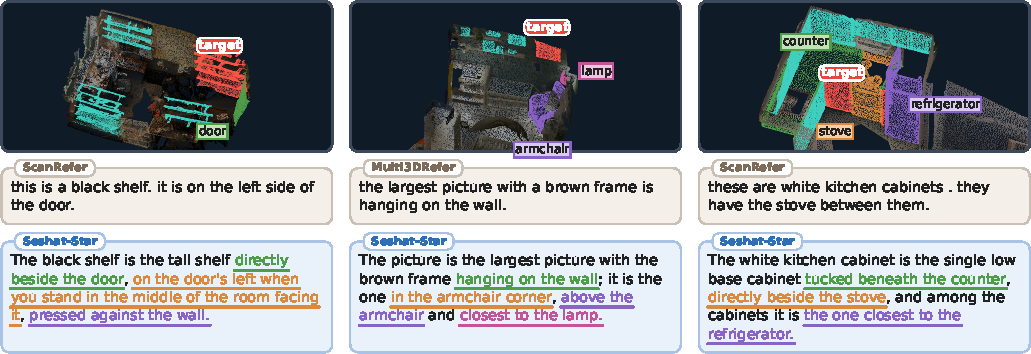
\includegraphics[width=\linewidth]{fig/examples.pdf}
\caption{\textbf{Three validation targets, in the annotator's words and in ours.}
Colour ties a clause to the predicate the blind reader returned for it and to the object it names; grey marks a clause the reader could not bind.
Each chip gives how many of the same-class candidates its predicate keeps.}
\label{fig:\currfilebase}
\end{figure*}
